\documentclass[titlepage ,12pt]{article}
\addtolength{\oddsidemargin}{-.875in}
\addtolength{\evensidemargin}{-.875in}
\addtolength{\textwidth}{1.75in}

\addtolength{\topmargin}{-.875in}
\addtolength{\textheight}{1.75in}


\usepackage[font=footnotesize]{caption}
\usepackage{verbatim}
\usepackage[section]{placeins}
\usepackage{comment}
%\usepackage{hyperref}

% This just adds lines between paragraphs
\usepackage[parfill]{parskip}

%This allows diagrams to be added
\usepackage{graphicx}


\usepackage{listings}
\usepackage{color}

\definecolor{dkred}{rgb}{0.6,0,0}
\definecolor{dkblu}{rgb}{0,0,0.6}
\definecolor{dkgreen}{rgb}{0,0.6,0}
\definecolor{gray}{rgb}{0.5,0.5,0.5}
\definecolor{mauve}{rgb}{0.58,0,0.82}

\lstset{showstringspaces=false,
		language=SQL,
        numbers=left,
        %frame=single,
        backgroundcolor=\color[RGB]{234,237,230},
        numberstyle=\tiny,
        basicstyle={\footnotesize\ttfamily\bfseries},
        %frameround=tttt,
        breaklines=true,
        keywordstyle=\color{dkblu},
        commentstyle=\color[RGB]{143,89,2},
        stringstyle=\color{dkgreen},
        identifierstyle=\color[RGB]{0,0,0},
		morekeywords={CreateMbrCache,mbr,FilterMbrWithin,MbrMinX,MbrMinY,MbrMaxX,MbrMaxY,Within,group_concat}        
        }



%opening
\title{CS270 Assignment 1 - Ski Lifts and Pistes}
\author{Si\^{o}n Griffiths - Sig2}

\begin{document}

\maketitle
\newpage
\tableofcontents
\clearpage


\section{Introduction}
This document provides an overview of my solution for the CS270 Ski Lifts and Pistes Assignment.
The problem given in the assignment brief is to analyse a set of data, normalise this data to a form suitable to be implemented in a relational database system, and provide a PostgreSQL implementation of this dataset.   

\section{Un-Normalized Structures}

Studying the dataset provided in the assignment brief, I have determined the un-normalized structure of the database (along with all repeating groups) to be as follows:
 
\textbf{Piste}(\underline{PisteName}, Grade, Length, Fall, Lifts, Open, LiftName, Type, Summit, Rise, LiftLength, Operating) \\ \\
(LiftName, Type, Summit, Rise, LiftLength, Operating) repeats for each lift
 \newline

The data is separated out into two tables which implies that some logical structuring has already been carried out. I have determined that Piste if the main entity of interest and all other attributes are in some way derivable from it. 

\subsection{Candidate Keys}
The following candidate keys have been identified: 

\subsubsection{Grade, Length, Fall}

A composite of the Grade, Length and Fall attributes would serve to uniquely identify a piste according to the data provided in the brief. Even though a composite of Grade + Fall or Length + Fall would also appear to uniquely identify a piste I have chosen to use a composite of all three as a candidate since all three together provide a key which is more unique. \\
The uniqueness of this composite key lies in the assumption that mountain slopes are of differing heights and gradients, and that the complexity of terrain on a mountain slope varies (Grade). \\
This candidate has not been chosen as primary key. It is usually best to avoid the use of composite keys as primary key if possible and there's always the possibility that 2 pistes could share similar slopes such that this candidate key would not be sufficient to differentiate between them.

\subsubsection{Lifts}

The Lifts attribute appears to be unique to each piste according to the dataset provided in the assignment brief. Each piste is served by a unique collection of lifts or lift, this would provide sufficient information to uniquely identify a piste. \\
This candidate key has not been chosen as primary key. Since some lifts serve a number of pistes it is possible to assume that a lift could be removed in the future, such that a number of pistes have the exact same set of lifts serving them, in this case the Lifts attribute would no longer be enough to uniquely identify a piste.

\subsubsection{A composite of all attributes}

Looking at the dataset, it is fairly safe to assume that the entire entry for a piste will always be unique. However, there are more suitable and concise choices available so this candidate has not been chosen as primary key.

\subsubsection{PisteName}

Each piste has a unique name. The PisteName is a single, concise entry that serves to uniquely identify a piste. Since this is the most concise and intuitive choice, it has been selected as the primary key for the un-normalized representation of the dataset. 


\subsection{Functional Dependencies}
The following functional dependencies have been identified: \\

\textbf{PisteName \begin{math}\rightarrow\end{math} Grade, Length, Fall, Lifts, Open}

The attributes Grade, Length, Fall, Lifts and Open can be considered functionally dependant on PisteName since they make no sense outside of the context of a Piste. None of these attributes on it's own is enough to identify a Piste. However, a PisteName is sufficient to derive any or all of these attributes. \\ 


\textbf{LiftName \begin{math}\rightarrow\end{math} Type, Summit, Rise, LiftLength, Operating}
 
Type, Summit, Rise, LiftLength and Operating can all be considered to be functionally dependant on LiftName. Similar to the situation with PistName and it's dependant attributes, LiftName can be used to resolve any of these attributes where as the attributes themselves in isolation cannot identify a Lift, or indeed any other attribute. 


\section{First Normal Form}
Having identified functional dependencies and chosen a primary key the structure can be normalised.

In order to bring the structure to first normal form, repeating groups must be removed from the relation as shown in the un-normalized structure in section 2 of this document. The primary key of the un-normalized structure is included in the key of the new relation. Doing so results in the following relations:

\textbf{Piste}(\underline{PisteName}, Grade, Length, Fall, Open) \\
\textbf{Lift}(\underline{LiftName, PisteName*}, Type, Summit, Rise, LiftLength, Operating)

Because of the functional dependency : \textbf{PisteName \begin{math}\rightarrow\end{math} Grade, Length, Fall, Lifts, Open}, all attributes in the Piste relation are derived via the PisteName.
Similarly, all attributes in Lift are derived via the LiftName, since \textbf{LiftName \begin{math}\rightarrow\end{math} Type, Summit, Rise, LiftLength, Operating}.
The structure is fairly close to the functional dependencies that were specified in the earlier section, but further work is required.

 


\section{Second normal Form}
In order to bring this representation to second normal form we must ensure that no attributes are partially dependant on parts of a composite primary key. The lift relation in the First Normal Form section above has it's attributes only dependant on the LiftName attribute and not on the PisteName foreign key that also makes up it's key. 

PisteName has to be removed from the Lift relation and in order to represent the many-to-many relationship between Pistes and Lifts, a new table is required. This new table will hold only a foreign key reference to both Lift and Piste via their primary keys. This results in the following relations: 

\textbf{Piste}(\underline{PisteName}, Grade, Length, Fall, Open) \\
\textbf{Lift}(\underline{LiftName}, Type, Summit, Rise, LiftLength, Operating) \\
\textbf{Serves}(\underline{PisteName*, LiftName*})

The structures are now fully compliant with the functional dependencies that were outlined in the previous sections.

\section{Third normal Form}
In order for a representation to be in third normal form, it must conform to first and second normal form and also transitive dependencies must be removed. No attributes should depend on anything but the primary key.

With the dataset used in this particular example third normal form requires no extra steps from second normal form since there are no transitive dependencies. 
\newpage  
\section{PostgreSQL Implementation}

\subsection{Attribute Types}
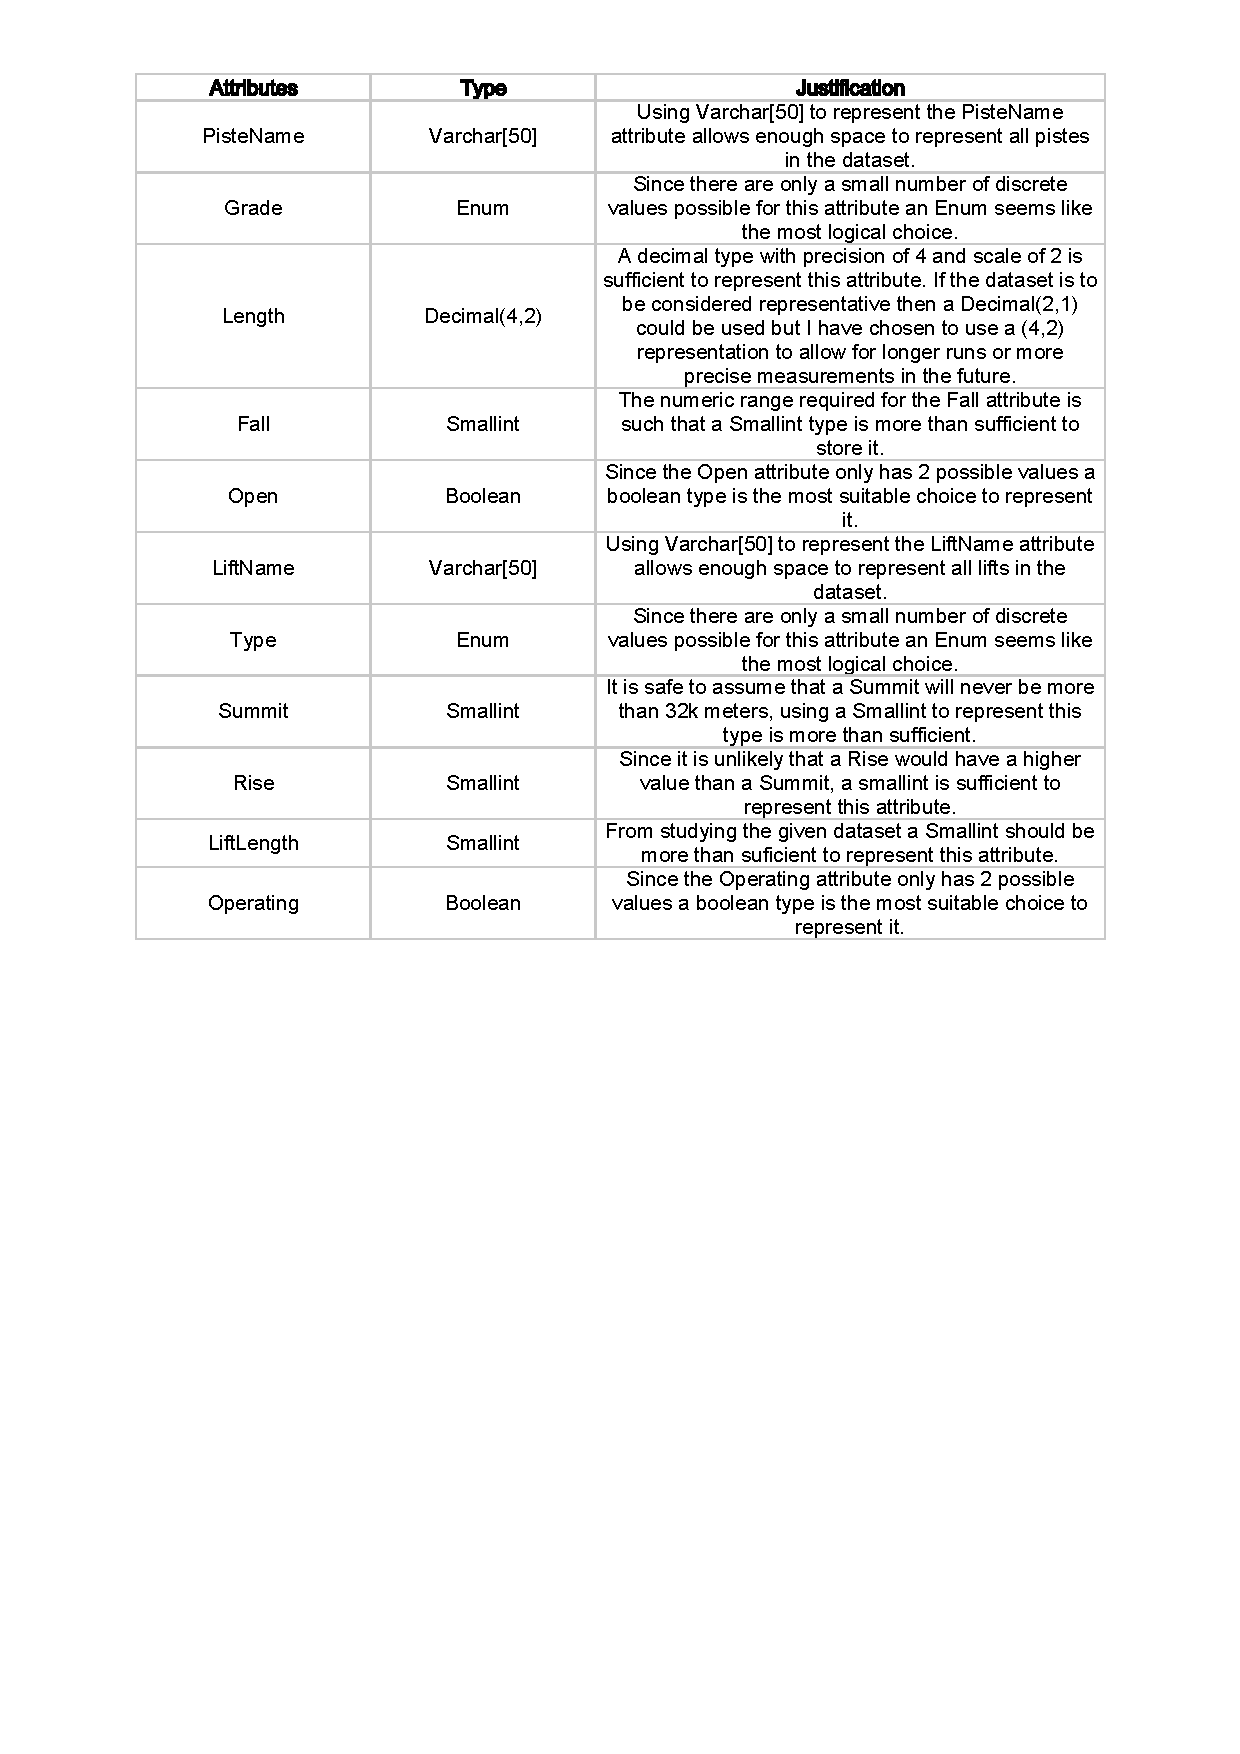
\includegraphics[width=0.9\textwidth]{images/types}
\subsection{SQL}
Implementing the database on the departmental computer system was achieved by running the following command for each of the files specified below. The SQL scripts themselves were uploaded to my university filestore. :
 

\begin{verbatim}
psql -h db.dcs.aber.ac.uk -U sig2 -d cs27020_13_14 < sql/filename.sql
\end{verbatim}

\subsection{Create Tables}
\lstinputlisting[breaklines=true]{SQL/create.sql}
\FloatBarrier



\newpage
\subsection{Inset Data}
\lstinputlisting[breaklines=true]{SQL/insert.sql}

\subsection{Queries}
\lstinputlisting[breaklines=true]{SQL/query.sql}

\subsection{Drop Tables}
\lstinputlisting[breaklines=true]{SQL/drop.sql}
\newpage
\subsection{Output}

The following screenshots show the output of running the SQL scripts detailed above.
\subsubsection{Create.sql}
\FloatBarrier
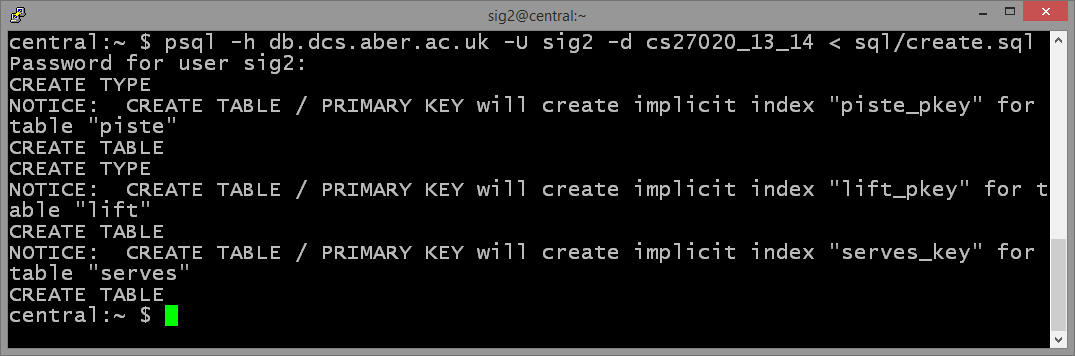
\includegraphics[width=0.9\textwidth]{images/create}\\
\subsubsection{Insert.sql}
\FloatBarrier
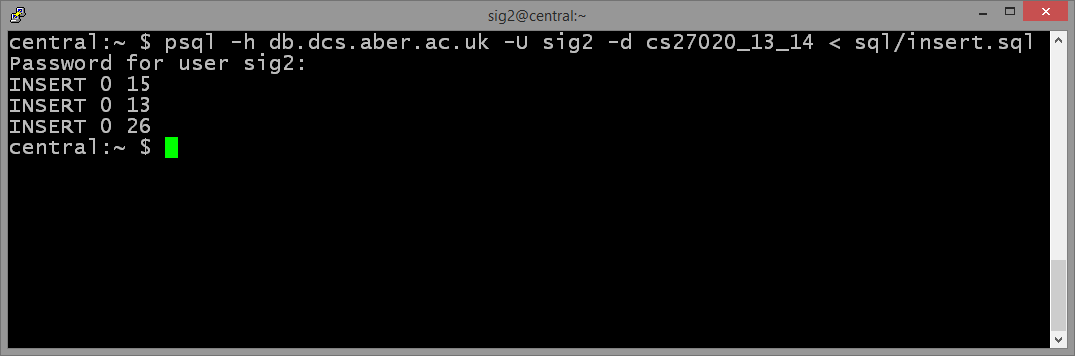
\includegraphics[width=0.9\textwidth]{images/insert}\\
\subsubsection{Query.sql}
\FloatBarrier
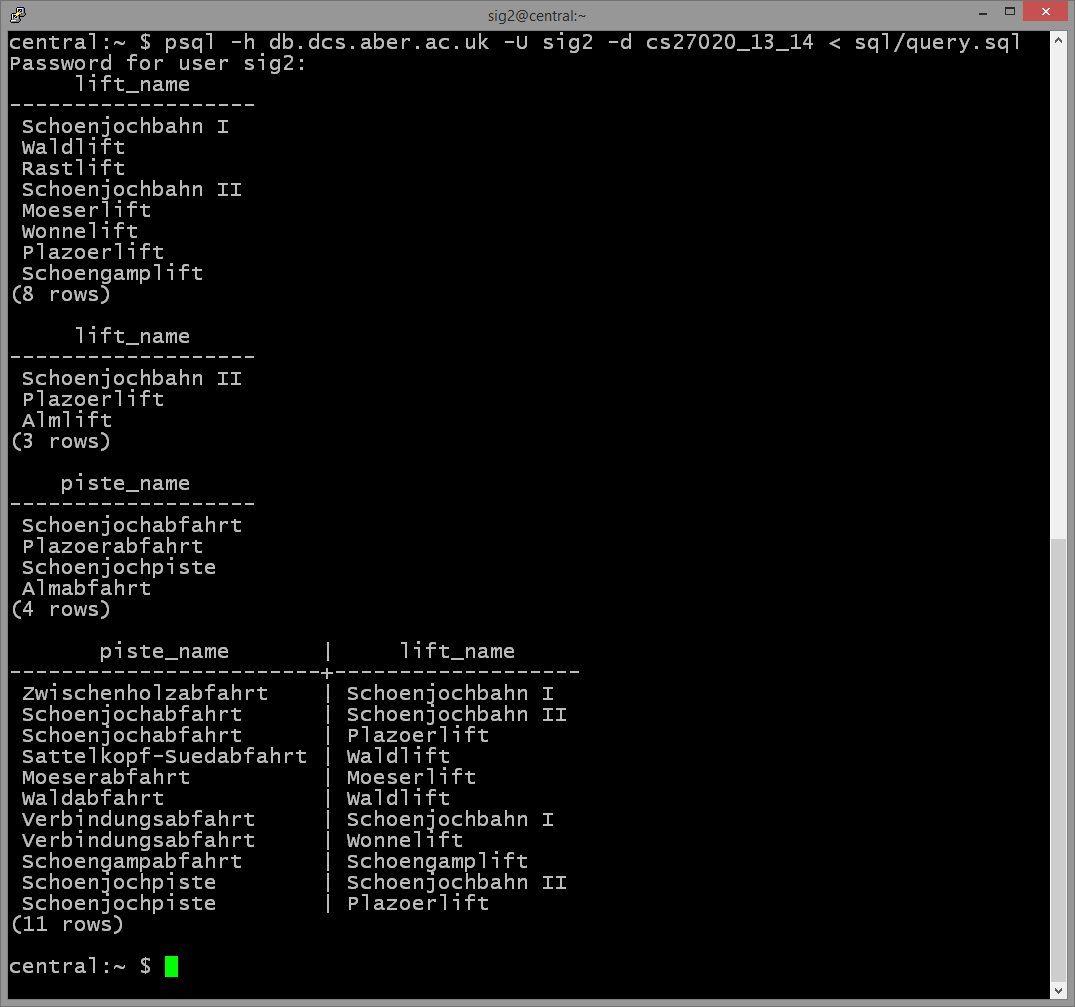
\includegraphics[width=0.9\textwidth]{images/query}\\
\subsubsection{Drop.sql}
\FloatBarrier
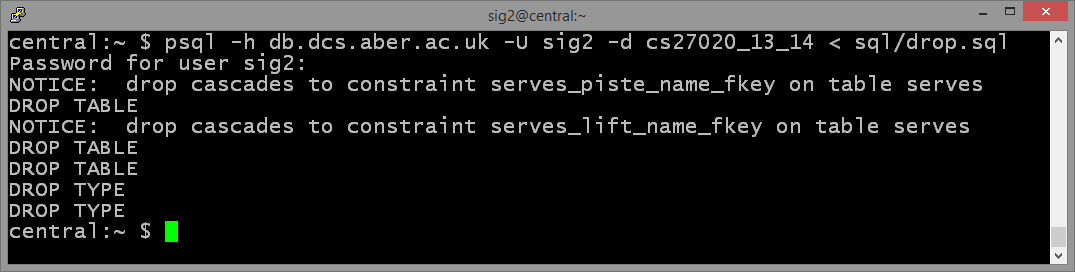
\includegraphics[width=0.9\textwidth]{images/drop}
\end{document}
